\documentclass{beamer}

\usetheme{Antibes}
\usepackage{pgfplots}
\usepackage{graphicx}
\title{CONTROL SYSTEMS}
\subtitle{Presentation}
\author{Aashrith-EE18BTECH11035}
\date{18th February}

\begin{document}

\begin{frame}
\titlepage    
\end{frame}


\begin{frame}{EC GATE-2016 Q.NO-45 }
In the feedback system given below G(s)= \(\frac{1}{s^2+2s}\) .\\
The step response of the closed-loop system should have minimum settling time and have no overshoot.

\begin{figure}
    \includegraphics[scale=0.5]{figs/Presentation.png}
\end{figure}

The required value of gain k to achieve this is \underline{\hspace{2cm}}

\end{frame}

\begin{frame}{Solution}
$Settling Time$: The time required for the transient's damped oscillations to
reach and stay within ±2\% of the steady-state value.\vspace{5mm}

$Overshoot$:The amount that the waveform overshoots the steady state, or final, value at the peak time, expressed as a percentage of the steady-state
value.\\
\vspace{5mm}
The Transfer function of the negative unity feedback system is given by \(\frac{G(s)}{1+G(s)H(s)}\) (Where G(s) is the open-loop gain of the system and H(s) is feedback gain) \\
\end{frame}
\begin{frame}
    
In the given Question G(s) = k x G(s) and H(s) = 1 .So, Transfer function of the whole feedback system is \(\frac{kG(s)}{1+kG(s)}\) \\
\bigskip
\\ By substituting G(s)=\(\frac{1}{s^2+2s}\) in the above equation we get
\bigskip
\\Closed loop Transfer function = \(\frac{k}{s^2+2s+K}\)
\end{frame}
\begin{frame}

\begin{figure}
    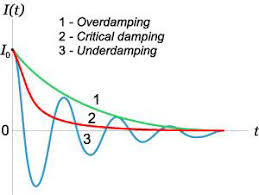
\includegraphics[scale=0.5]{figs/final1.jpeg}

    
\end{figure}

By observing the above figure,minimum settling time is obtained for Critical Damped System.\\
\bigskip
Also, Critically Damped System doesn't overshoot.
\end{frame}
\begin{frame}
\\ Transfer function of the Critical Damped System is given by
\(\frac{\omega_n^2}{s^2+2\zeta\omega_ns +\omega_n^2}\) (Where, \zeta=1 for Critical Damped System)\\
By comparing Obtained Transfer function \(\frac{k}{s^2+2s+K}\) and the general transfer function of Critical Damped System \(\frac{\omega_n^2}{s^2+2\zeta\omega_ns +\omega_n^2}\)\\
\vspace{5mm}\\
We get \omega_n^2 = K
\\ \omega_n = \sqrt{k}
\bigskip
\\ 2\zeta\omega_n s=2s
\\ \zeta = \(\frac{1}{\omega_n}\)
\\ \zeta = \(\frac{1}{\sqrt{K}}\)
\bigskip


\end{frame}

\begin{frame}
\\As, \zeta = 1\\
\vspace{5mm}\\
\(\frac{1}{\sqrt{K}}\) =1\\
\vspace{5mm}\\
K=1\\
\vspace{5mm}\\
Therefore, The value of K is 1.\\
\bigskip
The closed loop Transfer function is \(\frac{1}{s^2+2s+1}\)
\\ \(\frac{1}{s^2+2s+1}\) = \(\frac{1}{(s+1)^2}\)



\end{frame}
\begin{frame}
Laplace Transforms:
\bigskip
\\ \(\frac{1}{(s)}\) \longleftrightarrow u(t)
\bigskip
\\ \(\frac{1}{(s+1)}\) \longleftrightarrow e^{-t}u(t)
\bigskip
\\ \(\frac{1}{(s+1)^2}\) \longleftrightarrow te^{-t}u(t)
\bigskip
\\ In time domain \(\frac{1}{(s+1)^2}\) is equivalent to te^{-t}u(t)

\end{frame}
\begin{frame}
\\ Plot of Transfer function in time domain is:
\begin{figure}
    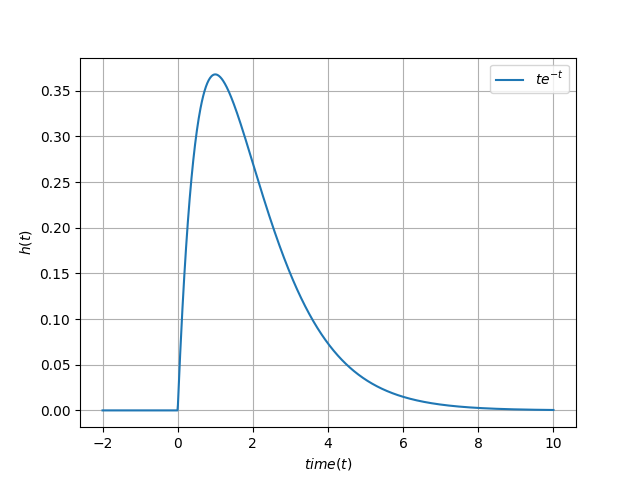
\includegraphics[scale=0.6]{figs/final.png}

    
\end{figure}
\end{frame}

\end{document}